\documentclass[
	% --- opções da classe memoir (https://www.ctan.org/pkg/memoir)
	12pt,    % tamanho da fonte
	oneside, % opção de impressão somente em anverso (frente). Oposto a opção twoside
	a4paper, % tamanho do papel
	% --- opções abtex2
	chapter=TITLE, % Títulos primários em maiúsculo
	section=TITLE, % Títulos secundários em maiúsculo
	sumario=tradicional, % Sumário tradicional memoir - alguns pontos customizados (abntex2-IFF.sty)
	% --- opções do pacote babel
	english, % adicional para hifenização correta de possíveis palavras em inglês
	brazil   % idioma padrão
] {abntex2}

% --- Pacotes essenciais
\usepackage{abntex2-IFF}
\usepackage[T1]{fontenc} % Exibição correta de alguns glifos de fonte
\usepackage[utf8]{inputenc} % Codificação padrão em utf8

\usepackage{url} % Utilização de url's no documento
\usepackage{indentfirst} % Primeiro parágrafo de cada seção também será indentado
\usepackage{graphicx} % Inclusão de figuras
\usepackage{multirow} % Múltiplas linhas em tabelas
\usepackage{booktabs} % Formatação de tabelas
\usepackage{longtable} % Utilização de tabelas longas
\usepackage{csquotes} % Facilita a colocação de textos entre aspas, como em citações através do comando \enquote.
\usepackage[linesnumbered, ruled, vlined, portuguese]{algorithm2e} % Utilização de algoritmos

\usepackage{xcolor} % Utilização de cores
\usepackage{amsmath} % Utilização de símbolos Matemáticos

% Configurações do pacote biblatex para Referências Bibliográficas
\usepackage[backend=biber, style=abnt, bibencoding=utf8, uniquename=init, giveninits, repeatfields]{biblatex}
\addbibresource{./referencias/referencias.bib}

% ==========================================================================================
% --------------------------------- INFORMAÇÕES DA CAPA ------------------------------------
% ==========================================================================================
% ---------------  Informações que constarão na CAPA ---------------
\titulo{Template para Trabalhos de Conclusão de Curso do Bacharelado em Sistemas de Informação do IFF}
\autor{Nome do discente} % Se houver mais de um autor, então adicionar uma quebra de linha (\\) após o primeiro nome 
\local{Itaperuna/RJ}
\data{2021}

% ==========================================================================================
% ---------------------------- INFORMAÇÕES DA FOLHA DE ROSTO -------------------------------
% ==========================================================================================
% --------------- Informações que constarão na FOLHA DE ROSTO ---------------
\orientador{Nome do orientador}
\coorientador{Nome do coorientador}
\preambulo{Trabalho de Conclusão de Curso apresentado no Instituto Federal Fluminense \emph{campus} Itaperuna como requisito parcial para conclusão do Curso de Bacharelado em Sistemas de Informação.}

% ==========================================================================================
% --------------------------- INFORMAÇÕES DA FOLHA DE APROVAÇÃO ----------------------------
% ==========================================================================================
% --------------- Informações que constarão na FOLHA DE APROVAÇÃO ---------------
% Caso queira uma instituição diferente no membro da banca, basta passar o parâmetro como 
% mostrado no membro B
\membrobancaA{Membro da banca A} % Definido em abntex2-IFF.sty - Instituição padrão IFF
\membrobancaB[UFF]{Membro da banca B} % Definido em abntex2-IFF.sty
\databanca{\today} % Definido em abntex2-IFF.sty

% Configurações para informações de metadados do PDF final
\makeatletter
\hypersetup {
	pdftitle={\@title},
	pdfauthor={\@author},
	pdfsubject={\imprimirpreambulo},
	pdfcreator={LaTeX with abnTeX2},
	colorlinks=false, % Não utiliza coloração nos links
	hidelinks % Oculta borda dos links no PDF gerado
}	
\makeatother


\begin{document}
	% ==========================================================================================
	% --------------------------------- ELEMENTOS PRÉ-TEXTUAIS ---------------------------------
	% ==========================================================================================
	\pretextual
	%---------------------- Mostra a CAPA (obrigatório)
	\imprimircapa
	
	%---------------------- Mostra a FOLHA DE ROSTO (obrigatório)
	\imprimirfolhaderosto
	
	%---------------------- Mostra a FOLHA DE APROVACAO (obrigatório)
	\imprimirfolhadeaprovacao

	%---------------------- FOLHA DE DEDICATÓRIA (opcional) -- Comente se desejar		
	\begin{dedicatoria}
		\vspace*{\fill}
		\hfill		
		\begin{minipage}[b][5cm]{.5\textwidth}
			\textit{Aos que acreditam que o \LaTeX\ é o melhor sistema tipográfico existente.}
		\end{minipage}		
	\end{dedicatoria}

	%---------------------- FOLHA DE AGRADECIMENTOS (opcional) -- Comente se desejar
	\begin{agradecimentos}				
		Agradeço a Deus pelo Dom da Vida...
	\end{agradecimentos}	

	%---------------------- FOLHA DE EPIGRAFE (opcional) -- Comente se desejar			
	\begin{epigrafe}	
		\vspace*{\fill}
		\hfill		
		\begin{minipage}[b][5cm]{.7\textwidth}
			\textit{E não vos conformeis com este século, mas transformai-vos pela renovação da vossa mente, para que experimenteis qual seja a boa, agradável e perfeita vontade de Deus.}\\
			(Bíblia Sagrada, Romanos 12:2)
		\end{minipage}
	\end{epigrafe}
	
	%---------------------- FOLHA DE RESUMO (obrigatório)	
	% Em Português
	\begin{resumo}
		Resumo em português.
		\vspace{\onelineskip}
		\noindent \\
		\textbf{Palavras-chave}: Latex. Template. Editoração de Texto.
	\end{resumo}
	
	% Em Inglês 
	\begin{resumo}[Abstract]
		English abstract.
		\vspace{\onelineskip}
		\noindent \\
		\textbf{Keywords}: Latex. Template. Text Editing.	
	\end{resumo}
	
	%---------------------- LISTA DE FIGURAS (opcional) -- Colocar somente se houver um número > 5 elementos	
	\renewcommand\listfigurename{LISTA DE FIGURAS}	
	\pdfbookmark[0]{Lista de Figuras}{lof}
	\listoffigures
	\cleardoublepage
	
	%---------------------- LISTA DE TABELAS (opcional) -- Colocar somente se houver um número > 5 elementos
	\renewcommand\listtablename{LISTA DE TABELAS}	
	%\pdfbookmark[0]{\listtablename}{lot}
	\listoftables
	\cleardoublepage

	%---------------------- LISTA DE ABREVIATURAS (opcional) -- Colocar somente se houver um número > 5 elementos
	\begin{siglas}
		\item[WYSIWYG:] What You See Is What You Get
		\item[WYSIWYM:] What You See Is What You Mean		
	\end{siglas}
	
	%---------------------- LISTA DE SÍMBOLOS (opcional) -- Colocar somente se houver um número > 5 elementos
	\begin{simbolos}
		\item[$ \Gamma $] Letra grega maiúscula Gama
		\item[$ \Lambda $] Letra grega maiúscula Lambda		
		\item[$ \zeta$] Letra grega minúscula zeta
		\item[$ \in $] Pertence
	\end{simbolos}	

	%---------------------- SUMÁRIO (obrigatório)
	\pdfbookmark[0]{\contentsname}{toc}	
	\tableofcontents*
	\cleardoublepage	
	
	% ==========================================================================================
	% --------------------------------- ELEMENTOS TEXTUAIS -------------------------------------
	% ==========================================================================================
	\textual	

	\chapter{Seção primária}\label{sec:primaria}

	Conteúdo da seção primária	
	
	\section{Seção secundária}\label{sec:secundaria}
	
	Conteúdo da seção secundária
	
	\subsection{Seção terciária}\label{sec:terciária}
	
	Conteúdo da seção terciária
	
	\subsubsection{Seção quaternária}\label{sec:quaternária}
	
	Conteúdo da seção quaternária
	
	\subsubsubsection{Seção quinária}\label{sec:quinária}
	
	Conteúdo da seção quinária
	
	% Repare que o título abaixo é um pouco mais longo, mas a entrada que aparece no sumário é somente
	\chapter{Imagens}\label{sec:imagens}
	\section{TeX}
	TeX (= tau epsilon chi, pronunciado como \enquote{tech}) é um sistema de tipografia criado por Donal Knuth em 1978. É popular no meio acadêmico, principalmente entre os físicos, matemáticos e cientistas da computação, devido sua sua capacidade de produzir fórmulas e símbolos matemáticos de uma maneira elegante.
	
	O principal motivo da criação do TeX foi a insatisfação de Knuth com a qualidade de impressão de seu segundo volume do magnum opus multivolume \textit{The Art of Computer Programming}~\footnote{\url{https://www.tug.org/whatis.html}}. A logo do \TeX \ pode ser vista na~\autoref{tex-logo}.
	
	\begin{figure}[htb]		
		\caption{Logo do \TeX}
		\label{tex-logo}
		\centering
		
\includegraphics[scale=.2]{./figuras/tex-logo.png}
		\legend{Fonte: \url{https://en.wikipedia.org/wiki/TeX}}
	\end{figure}
	
	\section{LaTeX}
	
	La\TeX(pronuncia-se \texttt{$<<$Lah-Tech$>>$} ou \texttt{$<<$Lay-Tech$>>$}) é um \textbf{conjunto de macros} criadas por Leslie Lamport para o processador de textos \TeX. O La\TeX \ fornece ao usuário comandos de alto nível, facilitando assim sua utilização.
	
	\begin{figure}[htb]		
		\caption{Logo do La\TeX}
		\label{latex-logo}
		\centering
		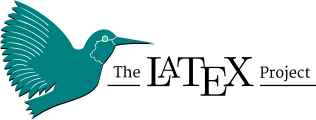
\includegraphics[scale=.5]{./figuras/latex-project-logo.png}
		\legend{Fonte: \url{https://en.wikipedia.org/wiki/LaTeX}}
	\end{figure}	

	\chapter{Tabelas}\label{sec:tabelas}
	
	\begin{table}[!htb]
		\centering
		\caption{As 10 Linguagens de Programação mais populares em Maio 2021}
		\label{tab:proglangs-v1}
		\vspace{3mm}
		\begin{tabular}{@{}llll@{}}
			\toprule[.1em]
			\textbf{Maio 2021}	& \textbf{Maio 2020}	& \textbf{Modificação}	& \textbf{Linguagem}\\
			\cmidrule{1-4}
					1			& 1     				&        					& C \\
					2			& 3     				& {\color{green}$\wedge$}	& python \\
					3			& 2     				& {\color{red}$\vee$}		& Java \\
					4			& 4     				& 							& C++ \\
					5			& 5     				& 							& C\# \\
					6			& 6     				& 							& Visual Basic \\
					7			& 7     				& 							& JavaScript \\
					8			& 14     				& {\color{green}$\wedge$}	& Assembly Language \\
					9			& 8     				& {\color{red}$\vee$}		& PHP \\				
					10			& 9     				& {\color{red}$\vee$}		& SQL \\				
			\bottomrule[.08em]
		\end{tabular}
		\fonte{Tiobe Index - \textcite{tiobeindex}}
	\end{table}
	
	Na \autoref{tab:proglangs-v1} podem ser vistas as 10 linguagens de programação mais populares em maio de 2021.	

	O abn\TeX~\footnote{\url{https://www.abntex.net.br/}} disponibiliza o comando \texttt{IBGEtab} que permite criar tabelas com formatação padronizadas de acordo com o IBGE (ABNT NBR 14724:2011~\footnote{\url{https://bit.ly/2T9jqaT}}). Na~\autoref{tab:prog-langs-v2} podemos ver a~\autoref{tab:proglangs-v1} no formato IBGE.


	\begin{table}[!htbp]
		\IBGEtab{
			\caption[Tabela Padrão IBGE]{As 10 Linguagens de Programação mais populares em Maio 2021}
			\label{tab:prog-langs-v2}
		}{
			\begin{tabular}{@{}llll@{}}
				\toprule[.1em]
				\textbf{Maio 2021}	& \textbf{Maio 2020}	& \textbf{Modificação}	& \textbf{Linguagem}\\
				\cmidrule{1-4}
						1			& 1     				&        					& C \\
						2			& 3     				& {\color{green}$\wedge$}	& python \\
						3			& 2     				& {\color{red}$\vee$}		& Java \\
						4			& 4     				& 							& C++ \\
						5			& 5     				& 							& C\# \\
						6			& 6     				& 							& Visual Basic \\
						7			& 7     				& 							& JavaScript \\
						8			& 14     				& {\color{green}$\wedge$}	& Assembly Language \\
						9			& 8     				& {\color{red}$\vee$}		& PHP \\				
						10			& 9     				& {\color{red}$\vee$}		& SQL \\				
				\bottomrule[.08em]
			\end{tabular}			
		}{\fonte{Tiobe Index - \textcite{tiobeindex}}}
	\end{table}

	\chapter{Algoritmos}\label{sec:algoritmos}
	\section{Busca Binária}
	
	O algoritmo de \textsf{busca binária} possui complexidade de tempo $O$(log $n$) e pode ser utilizado, por exemplo, para verificar de modo eficiente se um determinado \textit{array} ordenado possui um dado elemento fornecido.
	
	Um modo tradicional de implementarmos a busca binária é realizar a checagem do elemento central do \textit{subarray} e verificarmos se ele corresponde ao que estamos procurando, se sim, então o elemento procurado foi encontrado, caso contrário verificaremos se o elemento central é maior ou menor que o elemento procurado, caso seja maior, então a busca continua no \textit{subarray} esquerdo, senão no \textit{subarray} direito. No~\autoref{alg:binarysearch} podemos ver uma possível implementação deste raciocínio de forma iterativa.
	
	\vspace{.5cm}		
	\begin{algorithm}[H]
		\linespread{1}\selectfont
		\caption{\textsf{buscaBinaria(vet, tam, x)}}
		\label{alg:binarysearch}			
		\Entrada{Vetor (vet), tamanho do vetor (tam) e elemento a ser procurado (x)}
		\Saida{Posição onde o elemento se encontra ou -1 caso contrário}
		$a \gets 0$\;
		$b \gets tam - 1$\;
		$meio \gets -1$\;
		\Enqto{$(a \leq b)$} {
			meio = $(a + b) \; / \; 2$\;
			\Se{$(vet[meio] == x)$} {
				\Retorna meio \tcp*[l]{elemento encontrado}
			} 
			\eSe{$(vet[meio] < x)$} {
				$a \gets meio + 1$\;
			} {
				$b \gets meio - 1$\;
			}
		}
		\Retorna meio \tcp*[l]{elemento não encontrado}		
	\end{algorithm}
	\vspace{.5cm}		

	Em \textcite{laaksonen2017}, o autor traz uma excelente abordagem do algoritmo da \textsf{busca binária} e propõe um outro método de implementação. Também em \cite{programizsite} é realizada uma boa abordagem do algoritmo em suas versões iterativa e recursiva.
	
	\chapter{Material de Apoio}\label{sec:materia-apoio}
	Abaixo seguem algumas referências para se trabalhar com a classe \textsf{abn\TeX 2} (Da qual este template foi extendido) e da classe \textsf{memoir}, na qual o \textsf{abn\TeX 2} foi baseado. Também são mostradas referências para o pacote \textsf{biblatex-abnt}, no qual foi utilizado para gerenciar as referências deste template e que possui suporte para as regras de citação exigidas pela ABNT. 
	
	\begin{alineas}
		\item A classe \textsf{abn\TeX 2} 
			\begin{alineas}
				\item Site oficial: \url{https://www.abntex.net.br/}
				\item Repositório GitHub: \url{https://github.com/abntex/abntex2}
				\item Página \textsf{CTAN}: \url{https://www.ctan.org/pkg/abntex2}
			\end{alineas}
			
		\item A classe \textsf{memoir} 
			\begin{alineas}
				\item Página \textsf{CTAN}: \url{https://www.ctan.org/pkg/memoir}
			\end{alineas}

		\item O pacote \textsf{biblatex-abnt}
			\begin{alineas}
				\item Repositório GitHub: \url{https://github.com/abntex/biblatex-abnt}			
				\item Página \textsf{CTAN}: \url{https://www.ctan.org/pkg/biblatex-abnt}
			\end{alineas}
	\end{alineas}

	% ==========================================================================================
	% --------------------------------- ELEMENTOS PÓS-TEXTUAIS ---------------------------------
	% ==========================================================================================
	\postextual

	%---------------------- REFERÊNCIAS BIBLIOGRÁFICAS (obrigatório) 
	\linespread{1}
	\printbibliography[title={REFERÊNCIAS BIBLIOGRÁFICAS}]
	
	%---------------------- APÊNDICES ---------------------	
	\begin{apendicesenv}		
		\partapendices	
		\chapter{Primeiro Apêndice}
		\chapter{Segundo Apêndice}		
	\end{apendicesenv}
	
	%---------------------- ANEXOS ---------------------
	\begin{anexosenv}
		\partanexos
		\chapter{Primeiro Anexo}
		\chapter{Segundo Anexo}		
	\end{anexosenv}
	
\end{document}